

\section{Explain About Your Project}
A laptop selection and price prediction project mainly involves  using machine learning techniques to analyze various features of laptops and predict their prices based on those features and also selecting the best laptop among several laptops which are available in market. The goal is to build a model that can accurately predict the price of a laptop  and also choose one best laptop based on preferences and its specifications, such as the processor, RAM, storage capacity, display size, and other required information.
\par
Gather the  dataset from the online  websites like githud,kaggle etc.dataset contains the laptop specifications like Ram,processor,os,storage and display size etc..the selected dataset can includes  wide range of brands in market like Hp,lenovo,Dell etc..The dataset should cover a wide range of laptops from different brands, models, and price ranges.clean and preprocess the gathered data to increase its quality for training data to get accurate values of recommendations.This step involves handling missing values, removing duplicates and unneccesary data standardizing numerical features, and encoding categorical variables. It's important to procesthat can made the dataset is consistent and ready for further analysis.
\par 
After performing of data analysis on gathered dataset it helps in understanding of relationships between the different features of Laptop and Laptop prices.choosing  appropriate machine learning model among random forest,logistic regression,multiplelinear regression,k-nn algorithm etc.Based on the nature of gathered dataset we will choose best algorithm which gives more accurate values..
\paragraph{}
Once the model is trained using  collected dataset, it can be used to predict the price of a new laptop based on its specifications and also gives best laptop based on required specifications. Users can input the relevant features of a laptop into the trained model, and it will generate an estimated price as output .If we give required features to this model it will gives recommended laptop to them The predicted price can provide valuable insights for users when making decisions about laptop purchases.
\section{Data Set}
The dataset  collected from kaggle website contains information about various laptop specifications and their corresponding prices.THe dataset gives comprehensive view of different brands in market.
Name: this gives the information about different types of laptops in market. such as Dell, HP, Lenovo, Apple, etc. these features of the laptop influences prices of the laptop.
Ram: The amount of memory available for the laptop's operations. This feature represents the laptop's multitasking capability and influences its performance and price.
Storage: The storage capacity of the laptop, typically measured in gigabytes (GB) or terabytes (TB). This includes information about hard disk drives (HDD) or solid-state drives (SSD). The storage capacity affects the laptop's price and usability.
Display Size: The size of the laptop's screen, usually measured diagonally in inches. This feature helps users assess the laptop's  visual experience.
Processor: The type and specifications of the laptop's central processing unit (CPU). This feature includes information like the brand (Intel, AMD), the model (i5, Ryzen 7), the number of cores, and clock speed. The processor's performance significantly impacts the laptop's price.
Price: The actual price of the laptop. This is the target variable that the machine learning model aims to predict based on the other features.
os: The operating system is the software that manages computer hardware and software resources and provides a user interface for interacting with the computer.
\section{Prediction technique}
For laptop selection and price prediction, various machine learning techniques can be used. One common technique is regression analysis, which aims to predict a continuous numerical value, such as the price of a laptop. Regression models can capture the relationships between input features (such as processor, RAM, storage, etc.) and the output variable (price).
\paragraph{}
When it comes to the laptop selection process, the focus is typically on finding the most suitable laptop based on the user's specific needs and preferences. While price prediction is an important aspect of laptop selection, it is not the only factor considered. Therefore, the laptop selection process may involve various techniques beyond price prediction output variable is (name of the laptop).
, classification techniques may not be directly used for predicting the actual price of a laptop since price is a continuous numerical value. However, classification techniques can still be valuable for various related tasks and aspects of the project.
\paragraph{}
Classification algorithms can be used to identify the importance of different features in determining the price category of a laptop. By training a classifier on price categories and input features, you can obtain insights into which features have the most significant impact on the price classification. This information can help users understand the key factors driving laptop prices.
\paragraph{}
Decision Trees: Decision trees recursively split the dataset based on different features to create a tree-like model. Each leaf node represents a predicted value. Decision trees can handle both numerical and categorical features and capture non-linear relationships between features and price. However, they may suffer from overfitting if not properly regularized.
\paragraph{}
Random Forest: Random forest is an ensemble learning method that combines multiple decision trees. It averages the predictions of individual trees to produce a more robust and accurate prediction. Random forests can handle complex relationships and reduce overfitting by averaging predictions from different trees.
\section{Graphs}
\begin{lstlisting}[language=Python]
import numpy as np 
import pandas as pd 
import seaborn as sns 
sns.distplot(d["price(in Rs.)"])
plt.show()
\end{lstlisting}
 \begin{figure}[h]
\centering
 \footnotesize
 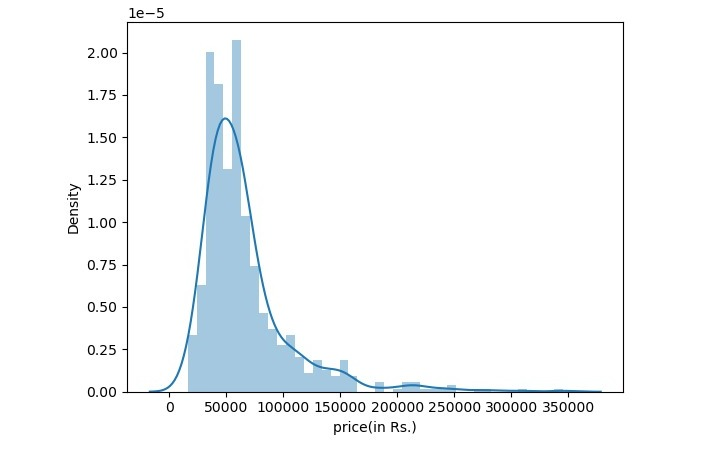
\includegraphics[width=6in]{1.png}
\caption{Analysis of price ranges for different Laptops}
\label{fig:dunnhalftone}
\end{figure} 
\begin{lstlisting}[language=Python]
import seaborn as sns
import pandas as pd
import  matplotlib.pyplot as plt
k=pd.read_csv("file2.csv")
plt.scatter(k['name'],k['ram'])
\end{lstlisting}
\vspace{5\baselineskip}
\begin{figure}[h]
\centering
 \footnotesize
 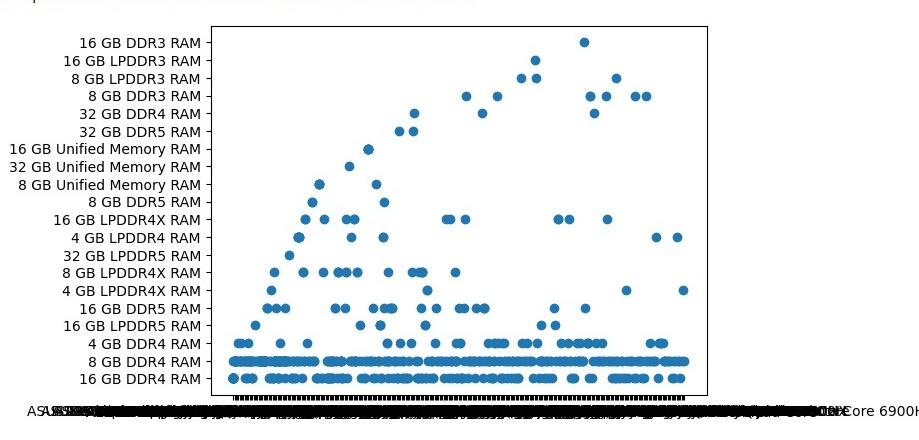
\includegraphics[width=6in]{2.png}
\caption{RAM Distribution}
\label{fig:dunnhalftone}
\end{figure} 
\begin{lstlisting}[language=Python]
import numpy as np
import pandas as pd
import  matplotlib.pyplot as plt
import seaborn as sns
p=sns.barplot(k['processor'],k['price(in Rs.)'])
\end{lstlisting}
 \begin{figure}[h]
\centering
 \footnotesize
 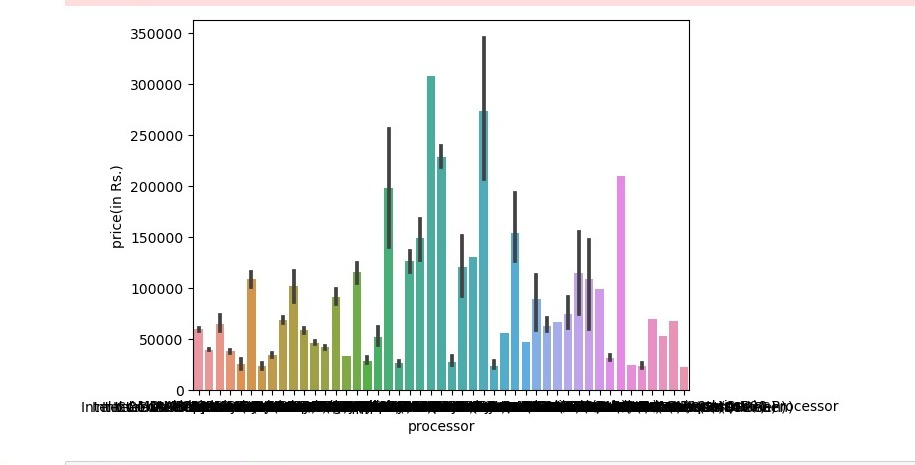
\includegraphics[width=6in]{3.png}
\caption{visual representation of the relationship between different processors and their prices.}
\label{fig:dunnhalftone}
\end{figure}
\begin{lstlisting}[language=Python]
import pandas as pd
import seaborn as sns
import  matplotlib.pyplot as plt
g=sns.JointGrid(x="rating",y="display(in inch)",data=d)
g=g.plot(sns.regplot,sns.distplot)
\end{lstlisting}
 \begin{figure}[h]
\centering
 \footnotesize
 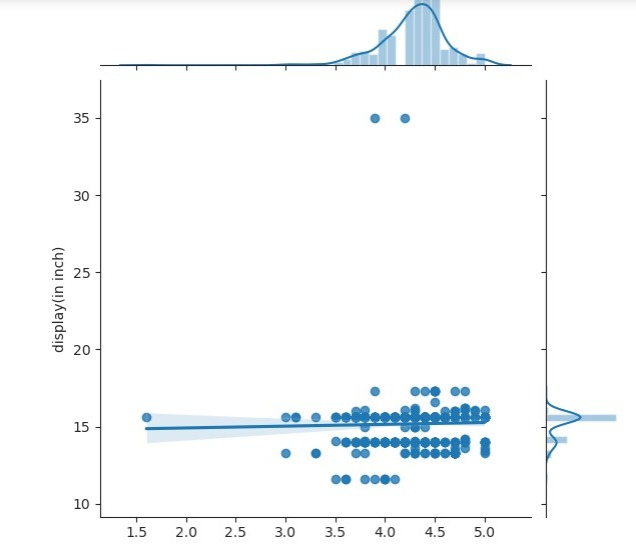
\includegraphics[width=4in]{4.png}
\caption{Distribution of ratings and display sizes}
\label{fig:dunnhalftone}
\end{figure} 


\begin{lstlisting}[language=Python]
import seaborn as sns
import pandas as pd
import  matplotlib.pyplot as plt
plt.figure(figsize=(12,6))
d.groupby('name').size().sort_values(ascending=False).head(5).plot(kind = 'bar',color = sns.color_palette('Paired'))
plt.xlabel('name of the laptop')
plt.ylabel('Number of Laptops')
plt.title('Top 5 most popular laptops brand')
plt.show()
\end{lstlisting}
\vspace{5\baselineskip}
\begin{figure}[h]
\centering
 \footnotesize
 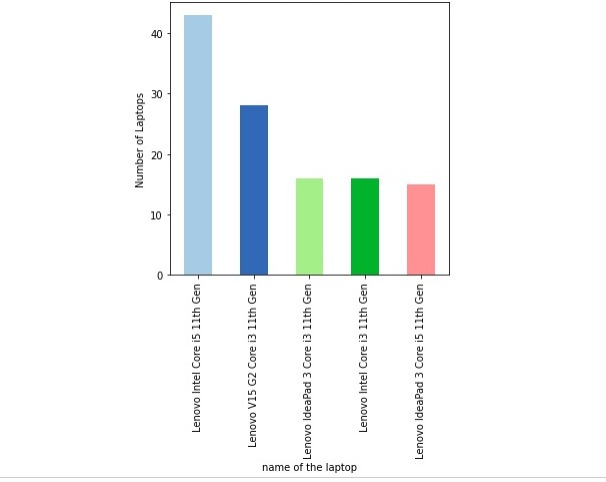
\includegraphics[width=4in]{5.png}
\caption{Top 5 most popular laptops brand}
\label{fig:dunnhalftone}
\end{figure} 
\begin{lstlisting}[language=Python]
import seaborn as sns
import pandas as pd
import  matplotlib.pyplot as plt
sns.boxplot(x="display(in inch)",y="rating",data=d)
plt.show()
\end{lstlisting}
\begin{figure}[h]
\centering
 \footnotesize
 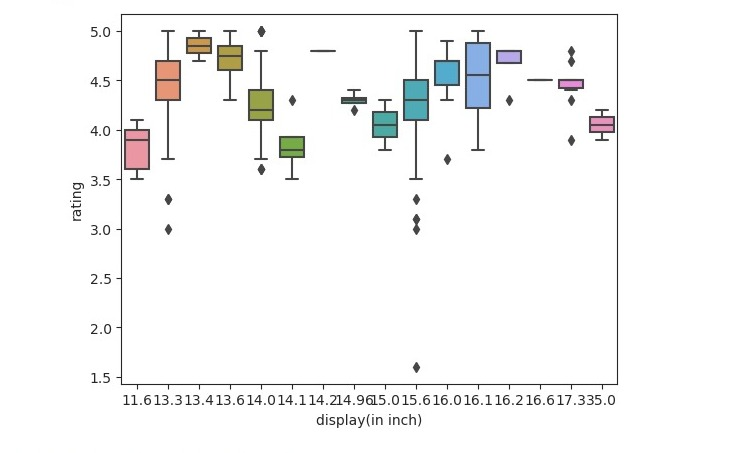
\includegraphics[width=4in]{7.png}
\caption{Example graph for box plot using seaborn }
\label{fig:dunnhalftone}
\end{figure} 
\begin{lstlisting}[language=Python]
import seaborn as sns
import pandas as pd
import  matplotlib.pyplot as plt
sns.violinplot(x=d["rating"])
plt.show()
\end{lstlisting}
\begin{figure}[h]
\centering
 \footnotesize
 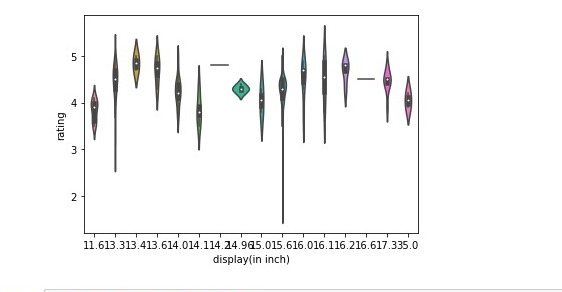
\includegraphics[width=4in]{8.png}
\caption{Distribution of ratings}
\label{fig:dunnhalftone}
\end{figure} 
\begin{lstlisting}[language=Python]
import seaborn as sns
import pandas as pd
import  matplotlib.pyplot as plt
plt.figure(figsize=(12,6))
d.groupby('ram').size().sort_values(ascending=False).plot(kind = 'bar',color = sns.color_palette('Blues'))
plt.xlabel('Ram Size in GB')
plt.ylabel('Number of Laptops')
plt.show()
\end{lstlisting}
\begin{figure}[h]
\centering
 \footnotesize
 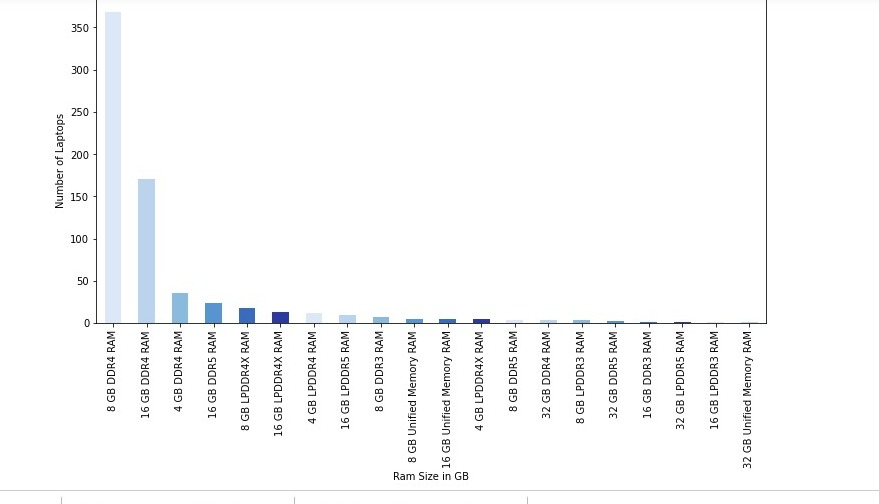
\includegraphics[width=4in]{9.png}
\caption{ graph shows the number of laptops for each RAM category}
\label{fig:dunnhalftone}
\end{figure} 

\begin{lstlisting}[language=Python]
import seaborn as sns
import pandas as pd
import  matplotlib.pyplot as plt
sns.set_style("ticks")
sns.pairplot(d)
plt.show()
\end{lstlisting}
\begin{figure}[h]
\centering
 \footnotesize
 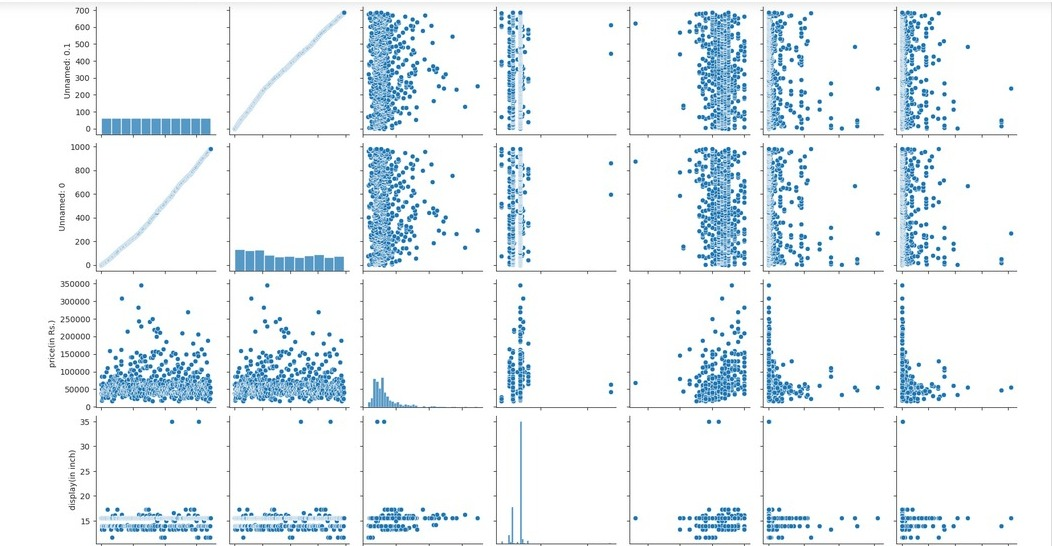
\includegraphics[width=4in]{11.png}
\caption{Relationships between variables}
\label{fig:dunnhalftone}
\end{figure} 
\begin{lstlisting}[language=Python]
import seaborn as sns
import pandas as pd
import  matplotlib.pyplot as plt
sns.distplot(d["price(in Rs.)"],kde=False)
plt.show()
\end{lstlisting}
\begin{figure}[h]
\centering
 \footnotesize
 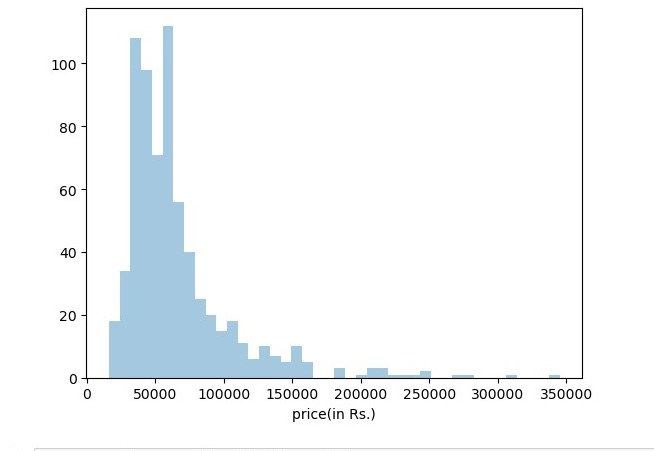
\includegraphics[width=4in]{12.png}
\caption{example graph of distplot}
\label{fig:dunnhalftone}
\end{figure} 

\section{Visualization} 
\begin{lstlisting}[language=Python]
plt.figure(figsize=(9,8))
sns.heatmap(d.corr(),square=True,annot=True,cmap="mako",center=0)
\end{lstlisting}
output:
\begin{figure}[h]
\centering
\footnotesize
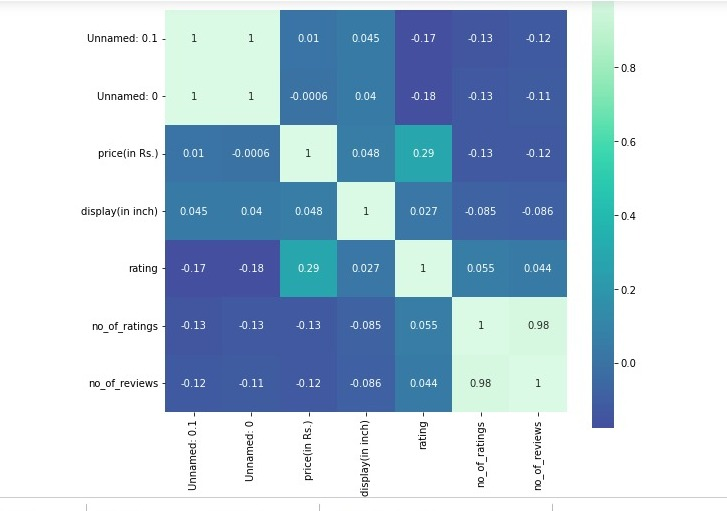
\includegraphics[width=8in]{13.jpeg}
\caption{Example for Heatmap}
\label{fig:unevenlight}
\end{figure}

 \begin{lstlisting}[language=Python]
 sns.regplot(x="rating",y="display(in inch)",data=d)
 plt.show()
 \end{lstlisting}
 \vspace{4\baselineskip}
 output:
\begin{figure}[h]
\centering
\footnotesize
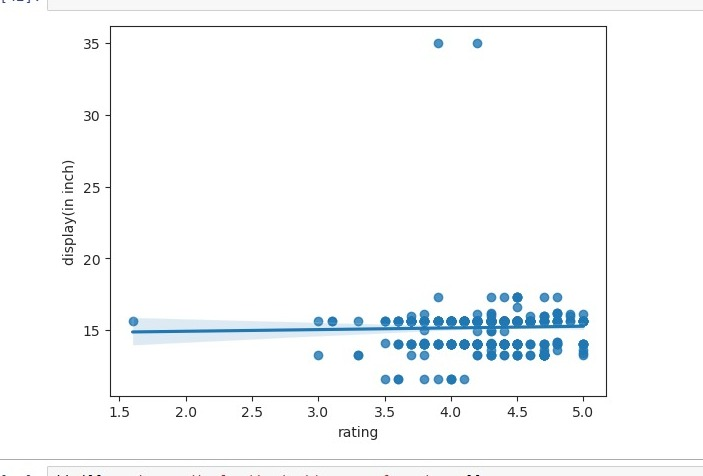
\includegraphics[width=4in]{15.png}
\caption{example graph for regplot}
\label{fig:unevenlight}
\end{figure}

\begin{lstlisting}[language=Python]
sns.distplot(d["rating"],hist=False)
plt.show()
 \end{lstlisting}
 output: 
\begin{figure}[h]
\centering
\footnotesize
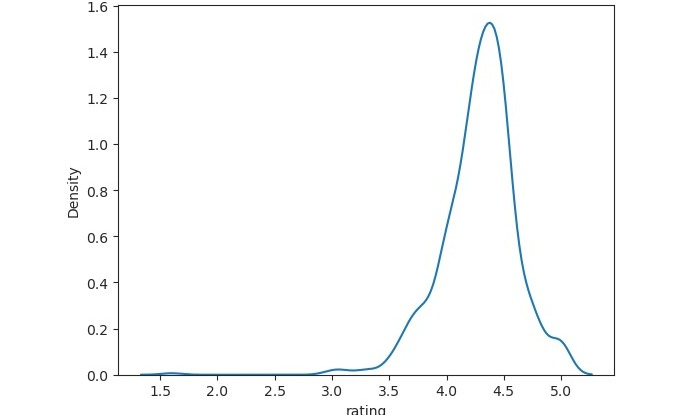
\includegraphics[width=5in]{16.png}
\caption{example graph for distplot}
\label{fig:unevenlight}
\end{figure}
 \vspace{4\baselineskip}

\begin{lstlisting}[language=Python]
sns.swarmplot(x="display(in inch)",y="rating",data=d)
plt.show()
 \end{lstlisting}
 output:
\begin{figure}[h]
\centering
\footnotesize
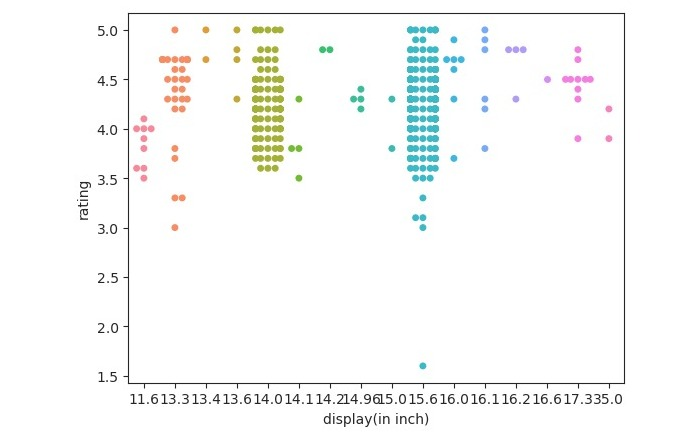
\includegraphics[width=6in]{17.jpeg}
\caption{  Example  of swarmplot}
\label{fig:unevenlight}
\end{figure}
This section contain minimum of 12 pages